\documentclass{beamer}\usepackage[]{graphicx}\usepackage[]{color}
%% maxwidth is the original width if it is less than linewidth
%% otherwise use linewidth (to make sure the graphics do not exceed the margin)
\makeatletter
\def\maxwidth{ %
  \ifdim\Gin@nat@width>\linewidth
    \linewidth
  \else
    \Gin@nat@width
  \fi
}
\makeatother

\definecolor{fgcolor}{rgb}{0.345, 0.345, 0.345}
\newcommand{\hlnum}[1]{\textcolor[rgb]{0.686,0.059,0.569}{#1}}%
\newcommand{\hlstr}[1]{\textcolor[rgb]{0.192,0.494,0.8}{#1}}%
\newcommand{\hlcom}[1]{\textcolor[rgb]{0.678,0.584,0.686}{\textit{#1}}}%
\newcommand{\hlopt}[1]{\textcolor[rgb]{0,0,0}{#1}}%
\newcommand{\hlstd}[1]{\textcolor[rgb]{0.345,0.345,0.345}{#1}}%
\newcommand{\hlkwa}[1]{\textcolor[rgb]{0.161,0.373,0.58}{\textbf{#1}}}%
\newcommand{\hlkwb}[1]{\textcolor[rgb]{0.69,0.353,0.396}{#1}}%
\newcommand{\hlkwc}[1]{\textcolor[rgb]{0.333,0.667,0.333}{#1}}%
\newcommand{\hlkwd}[1]{\textcolor[rgb]{0.737,0.353,0.396}{\textbf{#1}}}%
\let\hlipl\hlkwb

\usepackage{framed}
\makeatletter
\newenvironment{kframe}{%
 \def\at@end@of@kframe{}%
 \ifinner\ifhmode%
  \def\at@end@of@kframe{\end{minipage}}%
  \begin{minipage}{\columnwidth}%
 \fi\fi%
 \def\FrameCommand##1{\hskip\@totalleftmargin \hskip-\fboxsep
 \colorbox{shadecolor}{##1}\hskip-\fboxsep
     % There is no \\@totalrightmargin, so:
     \hskip-\linewidth \hskip-\@totalleftmargin \hskip\columnwidth}%
 \MakeFramed {\advance\hsize-\width
   \@totalleftmargin\z@ \linewidth\hsize
   \@setminipage}}%
 {\par\unskip\endMakeFramed%
 \at@end@of@kframe}
\makeatother

\definecolor{shadecolor}{rgb}{.97, .97, .97}
\definecolor{messagecolor}{rgb}{0, 0, 0}
\definecolor{warningcolor}{rgb}{1, 0, 1}
\definecolor{errorcolor}{rgb}{1, 0, 0}
\newenvironment{knitrout}{}{} % an empty environment to be redefined in TeX

\usepackage{alltt}

\usepackage{default}
\usepackage{animate} %need the animate.sty file 
\usepackage{graphicx}
%\graphicspath{{/home/sahir/Dropbox/jobs/laval/minicours/slides/}}
\usepackage{hyperref, url}
%\usepackage[round,sort]{natbib}   % bibliography omit 'round' option if you prefer square brackets
%\bibliographystyle{apalike}
\usepackage{biblatex}
\bibliography{bib.bib}
% Removes icon in bibliography
\setbeamertemplate{bibliography item}[text]

\usepackage[normalem]{ulem}

\setbeamertemplate{theorems}[numbered]



%\newtheorem{prop}{Proposition}
%\newenvironment{theoremc}[1]
%{\begin{shaded}\begin{theorem}[#1]}
%		{\end{theorem}\end{shaded}}
	
%\newtheorem{examplefirst}{Example}
%\newtheorem{examplesecond}{Example}
%\newenvironment<>{examplefirst}[1][]{%
%	\setbeamercolor{block title example}{bg=lightgray}%
%	\begin{example}#2[#1]}{\end{example}}
%\newenvironment<>{examplesecond}[1][]{%
%	\setbeamercolor{block title example}{fg=white,bg=blue!75!black}%
%	\begin{example}#2[#1]}{\end{example}}	

%\usepackage{amsthm}


\usepackage[figurename=Fig.]{caption}
\usepackage{subfig}
\usepackage{tikz, pgfplots,epsfig}
\usetikzlibrary{arrows,shapes.geometric}
\usepackage{color, colortbl,xcolor}
\definecolor{lightgray}{RGB}{200,200,200}
\definecolor{palegray}{RGB}{221,221,221}
\definecolor{myblue}{RGB}{0,89,179}
\usepackage{comment}
\setbeamercolor{frametitle}{fg=myblue}
\setbeamercolor{section in head/foot}{bg=myblue, fg=white}
\setbeamercolor{author in head/foot}{bg=myblue}
\setbeamercolor{date in head/foot}{bg=myblue}

\usepackage{shadethm}
%\colorlet{shadecolor}{blue!15}
\colorlet{shadecolor}{palegray}
%\setlength{\shadeboxrule}{.4pt}

\newshadetheorem{thm}{Theorem}
\newshadetheorem{defm}{Definition}
\newshadetheorem{exm}{Exercise}
\newshadetheorem{remarkm}{Remark}
%\definecolor{shadethmcolor}{HTML}{EDF8FF}
\definecolor{shadethmcolor}{RGB}{221,221,221}
%\definecolor{shaderulecolor}{HTML}{45CFFF}
\definecolor{shaderulecolor}{RGB}{0,89,179}
\setlength{\shadeboxrule}{.4pt}


\usepackage{array}
\newcolumntype{L}{>{\centering\arraybackslash}m{3cm}} % used for text wrapping in ctable
\usepackage{ctable}
\usepackage[utf8]{inputenc}
\usepackage{fontenc}
\usepackage{pifont}% http://ctan.org/pkg/pifont
\newcommand{\cmark}{\ding{51}}%
\newcommand{\xmark}{\ding{55}}%
\def\widebar#1{\overline{#1}}
\definecolor{whitesmoke}{rgb}{0.96, 0.96, 0.96}

\usepackage{amssymb}
\usepackage{amsmath}

\usepackage{bm}
\def\transpose{{\sf{T}}}
\def\E{{\skew0\bm{E}}}
\def\Xvec{{\skew0\bm{X}}}
\def\Xveca{{\skew0\bm{X}}_1}
\def\Xvecb{{\skew0\bm{X}}_2}

\def\Yvec{{\skew0\bm{Y}}}
\def\bmY{{\skew0\bm{Y}}}
\def\bmX{{\skew0\bm{X}}}
\def\bmy{{\skew0\bm{y}}}
\def\bmG{{\skew0\bm{G}}}
\def\bmS{{\skew0\bm{S}}}
\def\bmA{{\skew0\bm{A}}}
\def\bmB{{\skew0\bm{B}}}
\def\bmD{{\skew0\bm{D}}}
\def\bmI{{\skew0\bm{I}}}
\def\bmV{{\skew0\bm{V}}}
\def\bmU{{\skew0\bm{U}}}
\def\bv{{\skew0\bm{v}}}
\def\bw{{\skew0\bm{w}}}
\def\bmm{{\skew0\bm{m}}}
\def\bmzero{{\skew0\bm{0}}}
\def\bx{{\skew0\bm{x}}}
\def\xveca{{\skew0\bm{x}}_1}
\def\xvecb{{\skew0\bm{x}}_2}

\def\N{{\skew0\mathcal{N}}}
\def\T{{\small T}}

\def\mvec{{\skew0\bm{m}}}
\def\bmmu{{\skew0\bm{\mu}}}
\def\muvec{{\skew0\bm{\mu}}}
\def\balpha{{\skew0\bm{\alpha}}}
\def\bbeta{{\skew0\bm{\beta}}}
\def\bmtheta{{\skew0\bm{\theta}}}
\def\btheta{{\skew0\bm{\theta}}}

\def\cvec{{\skew0\mathbf{c}}}

\def\Xbar{\overline{X}}

\definecolor{lightgray}{rgb}{0.91,0.91,0.91}
\definecolor{purpleblue}{rgb}{0.50,0.50,1.00}



\usepackage{fontspec}
%\setsansfont{Fira Sans}
%\setmonofont{Fira Mono}
\setsansfont[ItalicFont={Fira Sans Light Italic},BoldFont={Fira Sans},BoldItalicFont={Fira Sans Italic}]{Fira Sans Light}
\setmonofont[BoldFont={Fira Mono Medium}]{Fira Mono}


\setbeamercolor{itemize item}{fg=myblue}
\setbeamertemplate{itemize item}[square]

\setbeamertemplate{navigation symbols}{\usebeamercolor[fg]{title in head/foot}\usebeamerfont{title in head/foot}\insertframenumber}
\setbeamertemplate{footline}{}

\newtheorem{proposition}[theorem]{Proposition}
\newtheorem{exercise}[theorem]{Exercise}

\titlegraphic{\hfill
\includegraphics[height=1cm]{mcgill_logo.png}}


%% You also use hyperref, and pick colors 
\hypersetup{colorlinks,citecolor=orange,filecolor=red,linkcolor=brown,urlcolor=blue}

\newcommand {\framedgraphiccaption}[2] {
	\begin{figure}
		\centering
		\includegraphics[width=\textwidth,height=0.8\textheight,keepaspectratio]{#1}
		\caption{#2}
	\end{figure}
}

\newcommand {\framedgraphic}[1] {
	\begin{figure}
		\centering
		\includegraphics[width=\textwidth,height=0.9\textheight,keepaspectratio]{#1}
	\end{figure}
}


\AtBeginSection[]{
	\begin{frame}
		\vfill
		\centering
		\begin{beamercolorbox}[sep=8pt,center,shadow=true,rounded=true]{title}
			\usebeamerfont{title}\insertsectionhead\par%
		\end{beamercolorbox}
		\vfill
	\end{frame}
}

\newcommand\Wider[2][3em]{%
	\makebox[\linewidth][c]{%
		\begin{minipage}{\dimexpr\textwidth+#1\relax}
			\raggedright#2
		\end{minipage}%
	}%
}



\newcommand{\blue}[1]{\textcolor{blue}{#1}}
\newcommand{\red}[1]{\textcolor{red}{#1}}
%\makeatother

\usepackage{xparse}
\NewDocumentCommand\mylist{>{\SplitList{;}}m}
{
	\begin{itemize}
		\ProcessList{#1}{ \insertitem }
	\end{itemize}
}
\NewDocumentCommand\mynum{>{\SplitList{;}}m}
{
	\begin{enumerate}
		\ProcessList{#1}{ \insertitem }
	\end{enumerate}
}
\newcommand\insertitem[1]{\item #1}

\newcommand\FrameText[1]{%
	\begin{textblock*}{\paperwidth}(0pt,\textheight)
		\raggedright #1\hspace{.5em}
\end{textblock*}}
\IfFileExists{upquote.sty}{\usepackage{upquote}}{}
\begin{document}
%\sffamily



%\title{Introduction to Regression Trees}
%\author{Sahir Bhatnagar \inst{1}}
%\author[shortname]{Sahir Rai Bhatnagar, PhD Candidate (Biostatistics) }
%\institute[shortinst]{Department of Epidemiology, Biostatistics and Occupational Health}

\title{Inference about a Population Mean ($\mu$)}
\subtitle{AAO unit 26; Baldi \& Moore, Ch 17}
\author{Sahir Bhatnagar and James Hanley}
\institute{
	EPIB 607\\
	Department of Epidemiology, Biostatistics, and Occupational Health\\
	McGill University\\
	
	\vspace{0.1 in}
	
	\texttt{sahir.bhatnagar@mcgill.ca}\\
	\texttt{\url{https://sahirbhatnagar.com/EPIB607/}}}

%\date

\maketitle

\section{The t distribution}

\frame{\frametitle{Inference for $\mu$ when $\sigma$ is not known}
	Up until now, all of our calculations have relied on us knowing the
	value of the population standard deviation ($\sigma$). It is rare that this is the case. \\ \ \\
	
	We now consider methods of inference for when $\sigma$ is unknown.
	\\ \ \\
	
	When $\sigma$ is unknown, we must estimate it from the data using $s$, the sample standard deviation.
}

\frame{\frametitle{Inference for $\mu$ when $\sigma$ is unknown}
	\begin{itemize}
		\item When the true variance was known, we performed our calculations
	using the standardization \[Z =
	\frac{\overline{y}-\mu}{\sigma/\sqrt{n}} \sim \mathcal{N}(0,1).\] \pause 
	\item We no longer can use this, so instead we use \[t =
	\frac{\overline{y}-\mu}{s/\sqrt{n}} \sim t_{(n-1)}\] which follows a
	\textbf{$t$-distribution} with $n-1$ degrees of freedom based on the $n$ values, $y_1,...,y_n$ in a simple random sample \pause
	\item There is a different $t$ distribution for each sample size. The
	degrees of freedom specify which distribution we use, and are
	determined by the denominator used in estimating $s$ which is $(n-1)$.
\end{itemize} }

\begin{frame}{A note about the conditions}
\begin{itemize}
	\setlength\itemsep{1em}
\item B\&M stress that the \textbf{first} of their conditions as \textit{very important}: \textit{we can regard} our data as a simple random sample (SRS) from  the population 
	\item The \textbf{second}, observations from the population have a \textit{\underline{Normal}} distribution with unknown mean parameter $\mu$ and unknown standard deviation parameter $\sigma$ less so
	\item \textit{In practice}, inference procedures \textit{can accommodate some deviations from
			the Normality condition} when the sample is large enough. (think CLT)
\end{itemize}
\end{frame}

%\frame{\frametitle{$t$ distributions}
%	\begin{figure}
%		\begin{center}
%			\epsfig{figure=Tables/psls_table_C.eps,scale=.35}
%		\end{center}
%	\end{figure}
%}

\frame{\frametitle{$t$ distributions} The $t$ distribution is
	symmetric, but has heavier tails than the Normal distribution. \\ \
	\\
	
	As the degrees of freedom increase (i.e., as $n$ increases), the
	$t$-distribution becomes more and more similar to a Normal
	distribution.\\ \ \\
	
	In fact, the quantiles/area under the curve are similar for
	$n\ge30$:
	\begin{center}
		\textbf{\underline{Quantiles}}\\ \vspace{.2cm}
		
		\begin{tabular}{c|cccc}
			Distribution & \multicolumn{4}{c}{Cumulative Probability}\\
			& 0.005 & 0.010 & 0.025 & 0.050\\ \hline
			Normal & -2.58 & -2.33 & -1.96 & -1.64\\
			$t$(50) & -2.68 & -2.40 & -2.01 & -1.68\\
			$t$(30) & -2.75 & -2.46 & -2.04 & -1.70\\
			$t$(10) & -3.17 & -2.76 & -2.23 & -1.81\\
		\end{tabular}
	\end{center}
} \frame{\frametitle{$t$ procedures} We can calculate CIs and
	perform significance tests much as before (example coming up
	soon).\\\ \\
	
	A significance test of a single sample mean using the $t$-statistic
	is called a \textcolor{blue}{one-sample $t$-test}. \\ \ \\
	
	Collectively, the significance tests and confidence-interval based
	tests using the $t$ distribution are called $t$ procedures. (Tests
	using the $Z$ statistic and the Normal distribution are a special
	case of these.) \\ \ \\
	
} \frame{\frametitle{Robustness of the $t$ procedures} A statistical
	procedure is said to be \textbf{robust} if it is insensitive to
	violations of the assumptions made. \\ \ \\
	\begin{itemize}
		\item Results of $t$ procedures (CIs, significance tests) are exact if the
		population from which the simple random sample was drawn is Normal. \pause
		\item $t$ procedures are not robust against \textit{extreme}
		skewness, particularly in small samples, since the procedures are
		based on using $\overline{x}$ and $s^2$ (which are sensitive to
		outliers).
		\item Recall: \textcolor{blue}{Unless there is a very compelling reason
			(e.g.~known/confirmed error in the recorded data), outliers should not be discarded.}
		\pause
	\end{itemize}
} \frame{\frametitle{Robustness of the $t$ procedures}
	\begin{itemize}
		\item $t$ procedures \textbf{are} robust against other forms
		of non-normality and, even with considerable skew, perform well when $n$ is large. Why?
		\pause
		\begin{itemize}
			\item When $n$ is large, $s^2$ is a good estimate of $\sigma^2$
			(recall that $s^2$ is unbiased and, like most estimates, precision
			improves with increasing sample size)
			\item CLT: $\overline{x}$ will be Normal when $n$ is large, even if the
			population data are not \item[]
		\end{itemize}
		\item ...so how large is large enough?
	\end{itemize}
}

\frame{\frametitle{Robustness of the $t$ procedures}
	\begin{itemize}
		\item When $n<15$ and the data are symmetric and do not exhibit outliers,
		$t$ procedures can be used \pause
		\item When $n\ge 15$ and the data do not exhibit extreme outliers or
		extreme skew, $t$ procedures can be used \pause
		\item When $n\ge 40$, $t$ procedures can be used even if the data are
		highly skewed
		\begin{itemize}
			\item Even when $\sigma$ is not known, can use tests/CIs
			based on the $Z$ statistic/Normal distribution rather than on the
			$t$ statistic/$t$ distribution. (Quantiles are very similar.)
			\item[]
		\end{itemize}
		\pause
		\item If the data are very skewed, there are other options to
		consider (whether $n$ is large or not):
		\begin{itemize}
			\item Transformations (be careful with interpretation!)
			\item Non-parametric models which do not assume any particular
			distribution of the data (we will study these in Part 5 of the
			course)
		\end{itemize}
	\end{itemize}
}

\frame{\frametitle{Confidence intervals for $\mu$ when $\sigma^2$ is
		unknown} When we must estimate the SE, the $(1-\alpha)$100\%
	confidence interval now formed is:
	\begin{eqnarray*}
		\hbox{CI:} & & \hbox{estimate} \pm \hbox{margin of error}\\
		& & =\overline{x} \pm t_{\alpha/2}s/\sqrt{n}
	\end{eqnarray*}
	where $t_{\alpha/2}$ is the quantile of the $t(n-1)$ distribution
	curve such that
	$P(-t_{\alpha/2} < t_{n-1} < t_{\alpha/2}) = 1-\alpha$. \\\ \\
	The CI is exactly correct when the distribution of the population
	data $x$ is Normal, and approximately correct otherwise. \\ \ \\
	
	Recall that with highly skewed distributions and small samples, the
	CLT may not provide a good approximation to the distribution of
	$\overline{x}$.}

%\frame{\frametitle{Confidence intervals for $\mu$ when $\sigma^2$ is
%		unknown}
%	\begin{figure}
%		\begin{center}
%			\epsfig{figure=Tables/psls_table_C.eps,scale=.35}
%		\end{center}
%	\end{figure}
%}

\frame{\frametitle{Confidence intervals for $\mu$ when
		$\sigma^2$ is unknown} Exercise: \\ Compute a 95\% and a 99\%
	confidence interval for the mean Wechsler score of children at
	Lake Wobegon assuming variance is unknown. \\ \ \\
	
	Recall, for a 95\% \textit{Normal} CI, we use $z_{\alpha/2} =
	z_{0.025} = 1.96$, and for a 99\% \textit{Normal} CI, we have
	$z_{\alpha/2} = z_{0.005} = 2.58$. What quantile values
	$t_{\alpha/2}$ are used to construct CIs if we don't know the
	variance? }

%\frame{\frametitle{Confidence intervals for $\mu$ when
%		$\sigma^2$ is unknown}
%	\begin{figure}
%		\begin{center}
%			\rotatebox{90}{\epsfig{figure=Tables/psls_table_C-marked1.eps,scale=.45}}
%		\end{center}
%	\end{figure}
%}

\frame{\frametitle{Confidence intervals for $\mu$ when $\sigma^2$ is
		unknown} Exercise: \\ Compute a 95\% and a 99\% confidence interval
	for the mean Wechsler score of children at
	Lake Wobegon assuming variance is unknown. \\ \ \\
	
	Components required to construct the CIs:
	\begin{itemize}
		\item $\overline{x} = 112.8$
		\item $s = \sqrt{160.4} = 12.7$
		\item $n=9$
		\item for a 95\% CI, we use $t_{\alpha/2} =
		t_{0.025} = 2.306$
		\item for a 99\% CI, we use $t_{\alpha/2} =
		t_{0.005} = 3.355$
\end{itemize} }


\begin{frame}{Inference about a population mean}
\textbf{(FREQUENTIST) INFERENCE for (PARAMETER)} $\mu$ -- the mean of an (effectively) infinite-size universe of $Y$ values --
based on the $n$ values, $y_1, \dots, y_n$ in an  SRS from that universe/population


`\textbf{\textit{Certain conditions apply}}'  \footnote{ B\&M stress that the \textbf{first} of their conditions `\textit{we can regard} our data as a simple random sample (SRS) from  the
	population' as \textit{very important};\\ { \scriptsize the \textbf{second}, `Observations from the population have a \textit{\underline{Normal}} distribution with unknown mean parameter $\mu$ and and unknown standard deviation parameter $\sigma$' less so: `\textit{In
			practice}, inference procedures \textit{can accommodate some deviations from
			the Normality condition} when the sample is large enough.'}}

\textbf{Point-estimate} of $\mu$  :  $\hat{\mu} = \bar{y}$  

\textbf{(Symmetric) Confidence Interval} CI for $\mu$ : $\bar{y} \pm ME,$\\
\ \  \  where the \underline{M}argin of \underline{E}rror (ME) is a 
\begin{itemize}
	\item
	$z$-multiple of SE \footnote{B\&M distinguish the SD of a statistic from its SE. They switch on p. 412: `When the standard deviation of a statistic is estimated from data, the result
		is called the standard error (SE) of the statistic. The SE  of the sample mean, $\bar{y}$
		is SEM = $s/\sqrt{n}.$'}, if $n$ is `large' AND \\ \ \\
	the Y values in the universe have a  `Normal' (Gaussian')  distribution or, if not, $n$ is large enough so that the Central Limit Theorem guarantees that the sampling distribution of possible $\bar{y}$'s of size $n$ from this universe is well enough approximated by a Gaussian distribution
	\item
	$t$-multiple of SE if `small' $n$ AND \\ \ \\
	the Y values in the universe have a  `Normal' (Gaussian')  distribution
\end{itemize}
\end{frame}




\section{t-distribution}

\begin{frame}{When and why we use the $t$-distribution}
\mylist{When $\sigma$ is unknown use $t$ distribution. \blue{but why?}; \pause the spread of the $t$ distribution is greater than $\mathcal{N}(0,1)$  }
\end{frame}



\begin{frame}[fragile]{Rejecting the Null ($H_0: \mu = \mu_0$) when $\sigma$ is known}
\[ \underbrace{z_{0.975}}_{\textrm{critical value}}=1.96 = \frac{\bar{x}-\mu_0}{\sigma/\sqrt{n}} \rightarrow \frac{1.96 \sigma}{\sqrt{n}} = \bar{x}-\mu_0   \] which means that to reject $H_0$ the difference between your sample mean and $\mu_0$ needs to be \blue{greater than $\frac{1.96}{\sqrt{n}}$ standard deviations} \pause
\begin{knitrout}\scriptsize
\definecolor{shadecolor}{rgb}{0.969, 0.969, 0.969}\color{fgcolor}

{\centering 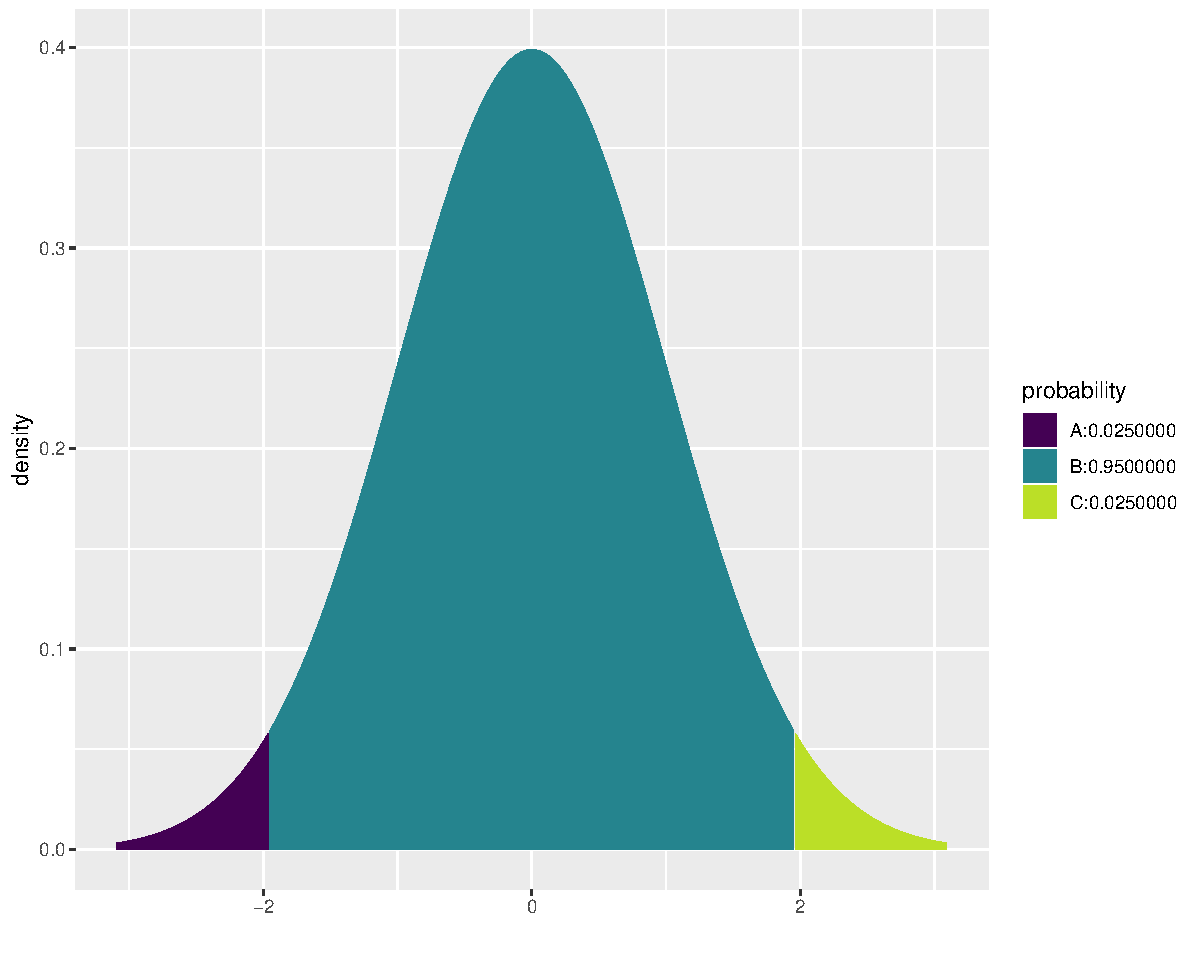
\includegraphics[width=.6\linewidth]{figure/unnamed-chunk-1-1} 

}



\end{knitrout}
\end{frame}



\begin{frame}[fragile]{Rejecting the Null ($H_0: \mu = \mu_0$) when $\sigma$ is unknown}
\[ \underbrace{t_{0.975,df=3}}_{\textrm{critical value}}=3.18 = \frac{\bar{x}-\mu_0}{s/\sqrt{n}} \rightarrow 3.18 \frac{s}{\sqrt{n}} = \bar{x}-\mu_0   \] which means that to reject $H_0$ the difference between your sample mean and $\mu_0$ needs to be \blue{greater than $\frac{3.18}{\sqrt{n}}$ standard deviations} \pause
\begin{knitrout}\scriptsize
\definecolor{shadecolor}{rgb}{0.969, 0.969, 0.969}\color{fgcolor}

{\centering 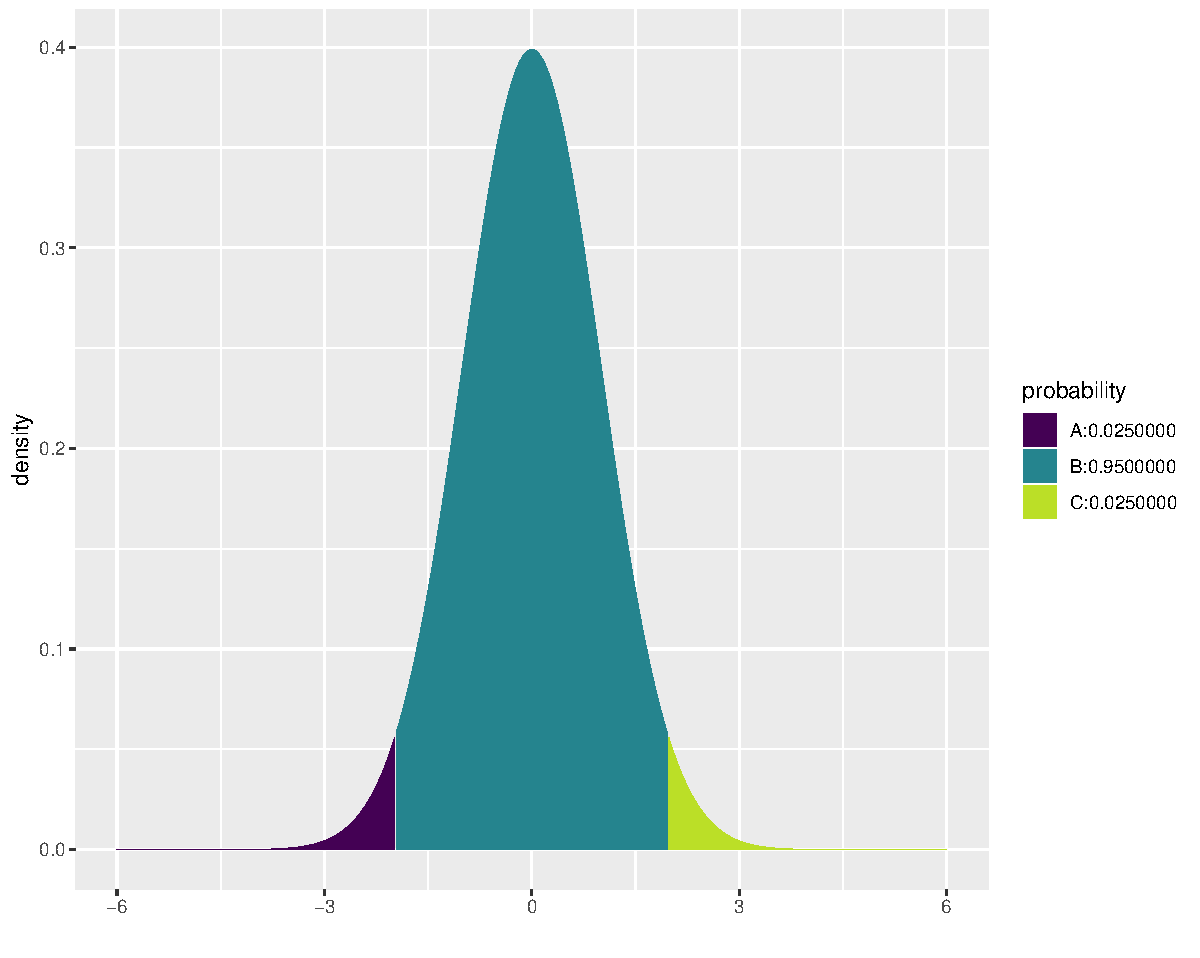
\includegraphics[width=.6\linewidth]{figure/unnamed-chunk-2-1} 

}



\end{knitrout}
\end{frame}




\begin{frame}{Summary of $t$ distribution}
\mylist{Its harder to reject the null when using the $t$ distribution; \pause This is due to our uncertainty about the estimated variance ;\pause Larger samples lead to more accurate estimates of $\sigma$; \pause This is reflected in the fact that there is a different $t$ distribution for each sample size  ; \pause As $n \rightarrow \infty$, sample variance $S$ gets closer to $\sigma$; \pause As degrees of freedom increase, $t$ distribution gets closer to Normal distribution}
\end{frame}


\begin{frame}{Summary of $t$ distribution}
Sample size increases $\rightarrow$ degrees of freedom increase $\rightarrow$ $t$ starts to look like $\mathcal{N}(0,1)$
\begin{knitrout}\scriptsize
\definecolor{shadecolor}{rgb}{0.969, 0.969, 0.969}\color{fgcolor}

{\centering 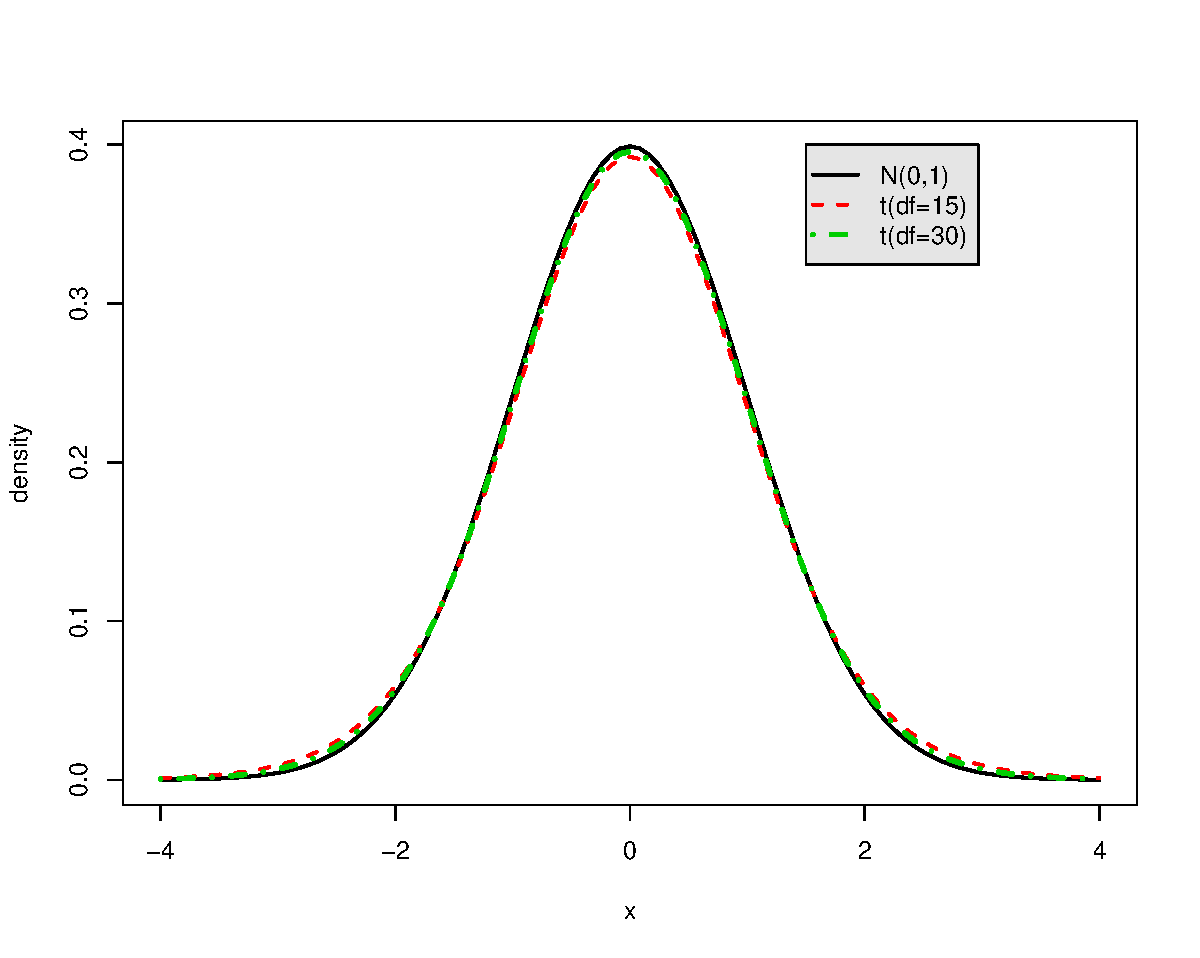
\includegraphics[width=.6\linewidth]{figure/unnamed-chunk-3-1} 

}



\end{knitrout}
\end{frame}


\begin{frame}{As df (proxy to the sample size) increases $\ldots$}
Recall that the 97.5th quantile of the $\mathcal{N}(0,1)$ is $Z=1.96$ \pause
\begin{center}
\begin{tabular}{c|c}
$df$ & $t_{0.975,df}$\\
\hline
3 & 3.1824463\\
5 & 2.5705818\\
30 & 2.0422725\\
50 & 2.0085591\\
100 & 1.9839715\\
250 & 1.9694984\\
500 & 1.9647198
\end{tabular}
\end{center}

\end{frame}




\end{document}
